%!TEX root=../GaugeCNNTheory.tex

\section{مدل اسباب‌بازی: کانولوشن‌های موبیوس هم‌متغیر انعکاس}
\label{sec:mobius_conv}

برای ملموس‌تر کردن ملاحظات نظری بخش‌های قبلی، اکنون به یک نمونه کاربرد می‌پردازیم.
در حالی که از اهمیت عملی فوری برخوردار نیست، کانولوشن‌های $\GM$ روی نوار موبیوس یک مدل اسباب‌بازی مناسب هستند زیرا هندسه آن و نظریه نمایش درگیر به‌ویژه ساده است.
به دلیل غیرجهت‌پذیر بودن آن، چارچوب‌های مرجع فقط می‌توانند (به‌طور هموار) تا حد انعکاس‌ها ترجیح داده شوند.
همانطور که انتظار می‌رود، \CNN های مستقل از مختصات، با اعمال توابع الگوی هم‌متغیر انعکاس، از پیاده‌سازی ساده‌لوحانه وابسته به مختصات بهتر عمل می‌کنند.
علاوه بر این نشان داده می‌شود که آنها تحت عمل گروه ایزومتری نوار موبیوس هم‌متغیر هستند.

\etocsettocdepth{3}
\etocsettocstyle{}{} % from now on only local tocs
\localtableofcontents

بخش~\ref{sec:mobius_geometry} در ادامه هندسه نوار موبیوس مسطح را مورد بحث قرار می‌دهد.
به دلیل پیچ آن، گروه ساختار آن نمی‌تواند بیش از گروه انعکاس~$G=\Flip$ کاهش یابد، به‌طوری که باید اطلس $\Flip$ از گیج‌ها را همانطور که در شکل~\ref{fig:mobius_conv_gauges} نمایش داده شده، در نظر گرفت.
گروه ایزومتری توسط چرخش‌ها در امتداد نوار داده می‌شود و تبدیل‌های گیج با مقادیر $\Flip$ را القا می‌کند.
میدان‌های ویژگی مستقل از مختصات $\RM$، که برخی از آنها در بخش~\ref{sec:mobius_representations} معرفی می‌شوند، لزوماً باید مطابق با نمایشی از گروه انعکاس تبدیل شوند.
بخش~\ref{sec:mobius_cnn_ops_analytical} عملیات شبکه کانولوشنی مستقل از جهت‌گیری را مورد بحث قرار می‌دهد.
این به‌ویژه مفهوم کرنل‌های $G$-راهبری‌پذیر را روشن می‌کند اما همچنین بایاس‌های هم‌متغیر انعکاس و غیرخطی‌ها را پوشش می‌دهد.
پیاده‌سازی عددی خانواده مدل پیشنهادی در بخش~\ref{sec:mobius_experiment_main} مورد بحث و ارزیابی قرار می‌گیرد.
کد به‌طور عمومی در \url{https://github.com/mauriceweiler/MobiusCNNs} در دسترس است.


%!TEX root=../GaugeCNNTheory.tex

\subsection{هندسه نوار موبیوس}
\label{sec:mobius_geometry}

منیفلد $M$ مورد بررسی نوار موبیوس مسطح با مرز است همانطور که در شکل~\ref{fig:weight_sharing_ambiguity} (راست) نشان داده شده است.
می‌توان آن را به‌عنوان ساخته شده از زیرمجموعه مستطیلی $[0,X] \times [0,Y]$ از $\R^2$ و چسباندن دو انتهای مقابل به‌شکل پیچ‌خورده در نظر گرفت.
با این تعریف، نوار موبیوس متریک کانونی $\R^2$ را به ارث می‌برد که آن را با ساختار ریمانی مجهز می‌کند.
متریک به‌ویژه اتصال لوی-چیویتا و در نتیجه نگاشت‌های نمایی و انتقال‌دهنده‌های موازی را مشخص می‌کند که در ادامه بیشتر مورد بحث قرار می‌گیرند.

\begin{figure}
	\centering
	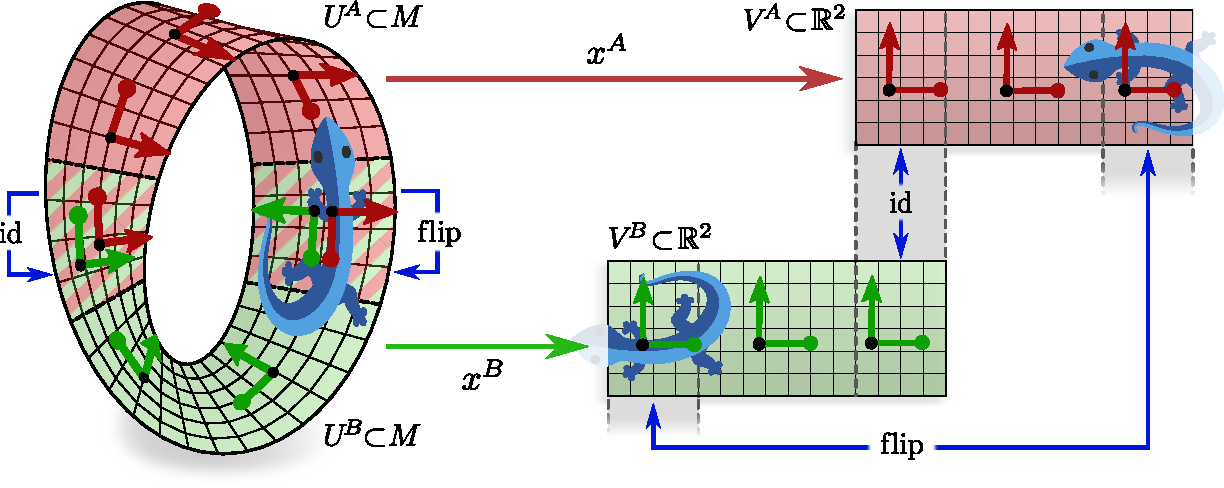
\includegraphics[width=\columnwidth]{figures/mobius_conv_gauges.pdf}
	\vspace*{.5ex}
	\caption{\small
		هندسه مسطح نوار موبیوس امکان زیرمجموعه‌های محلی را فراهم می‌کند که می‌توانند به‌طور ایزومتریک با زیرمجموعه‌های متناظر از~$\R^2$ شناسایی شوند.
		ما اطلسی ایزومتریک را ثابت می‌کنیم که از دو چارت $x^A$ و $x^B$ روی $U^A$ (قرمز) و $U^B$ (سبز) تشکیل می‌شود که کل نوار را می‌پوشانند.
		گیج‌های $\psi_p^X = \hat{d}x_p^X: \TpM \to \R^d$ برای $p\in U^A$ به‌عنوان دیفرانسیل‌های چارت القا می‌شوند.
		به دلیل پیچ نوار موبیوس، توابع گذار $g_p^{BA}$ در یکی از نواحی همپوشان بدیهی خواهند بود، در حالی که ناحیه دیگر لزوماً بین گیج‌ها از طریق انعکاس‌های~$s$ گذار خواهد کرد.
		اطلس انتخاب شده از چارت‌ها بنابراین $\Flip$-اطلسی از گیج‌ها را القا می‌کند و $\Flip$-ساختار متناظر $\RM$ را مستلزم می‌شود که از دو چارچوب منعکس‌شده در هر نقطه از~$M$ تشکیل می‌شود.
		هر یک از چارت‌های $x^X$ میدان چارچوب محلی هموار را القا می‌کند که توسط پایه‌های مختصاتی
		$\Big[\frac{\partial}{\partial x_i^X} \mkern-1mu\big|_p \Big] \raisebox{-2pt}{$\rule{0pt}{11pt}_{i=1}^d$}$
		داده می‌شود.
		انعکاس در توابع گذار در یک همپوشانی در انعکاس چارچوب‌ها نمایان می‌شود.
		{
			\\ \color{gray} \scriptsize
			(مارمولک‌ها تحت مجوز \lr{Creative Commons Attribution 4.0 International}
			\href{https://github.com/twitter/twemoji/blob/gh-pages/LICENSE-GRAPHICS}{\underline{\lr{license}}}
			با مجوز \lr{Twitter} اقتباس شده‌اند.)
		}
	}
	\label{fig:mobius_conv_gauges}
\end{figure}

اولین سؤالی که در ساخت \CNN مستقل از مختصات باید پاسخ داد این است که تا چه حد انتخاب چارچوب‌های مرجع مبهم است.
با توجه به متریک ریمانی روی نوار، می‌توانیم توجه خود را به چارچوب‌های متعامد محدود کنیم.
علاوه بر این می‌توان یکی از دو جهت \emph{در امتداد} نوار را متمایز کرد تا چرخش چارچوب‌های مرجع را با تراز کردن محورهای اول آنها با این جهت (به‌طور هموار) رفع ابهام کرد.
این ما را با ابهام دست‌گردی چارچوب باقی می‌گذارد، با دو جهت‌گیری که متناظر با دو جهت ممکن محور دوم چارچوب عمود بر نوار هستند.
نوار موبیوس به‌عنوان منیفلد غیرجهت‌پذیر، انتخاب سراسری هموار (یا حتی پیوسته) جهت‌گیری‌های چارچوب را نمی‌پذیرد.
برای به دست آوردن شهودی از این گزاره، تلاش برای ساخت میدان چارچوب هموار با انتخاب چارچوب دلخواه در موقعیت تصادفی و گسترش هموار این انتخاب روی کل نوار را در نظر بگیرید.
پس از یک دور کامل در اطراف نوار، چارچوب‌های ساخته‌شده ناگزیر نسبت به چارچوب‌های اولیه منعکس خواهند شد و بنابراین با هموار بودن مطلوب در تناقض خواهند بود.
بنابراین از نظر توپولوژیکی تعریف $\{e\}$-ساختار، یعنی میدان سراسری هموار چارچوب‌ها، روی نوار موبیوس \emph{غیرممکن} است.
بنابراین ما با گروه ساختار غیرقابل کاهش
\begin{align}
	G \,=\, \Flip \,\cong\, \Z/2\Z \,,
\end{align}
که انعکاس چارچوب‌ها را مدل می‌کند، باقی می‌مانیم.
گروه انعکاس فقط شامل دو عنصر است، همانی $e$ و انعکاس $s$، که طبق جدول ضرب ساده زیر ترکیب می‌شوند:
\begin{align}\label{eq:reflection_multiplication_table}
	\begin{tabular}{c|c@{\hspace{8pt}}c}
		& $e$ & $s$ \\ \hline
		$e$ & $e$ & $s$ \\
		$s$ & $s$ & $e$
	\end{tabular}
\end{align}
تنها گزاره غیربدیهی در این جدول این است که دو انعکاس یکدیگر را خنثی می‌کنند، یعنی $s^2=e$، یا به‌طور معادل، $s^{-1}=s$.
با توجه به غیرقابل کاهش بودن گروه ساختار $\Flip$، در ادامه باید $\Flip$-ساختار متناظر $\RM$ را در نظر بگیریم که از دو چارچوب با دست‌گردی مخالف در هر نقطه روی نوار موبیوس تشکیل می‌شود.

%!TEX root=../GaugeCNNTheory.tex

برای کدگذاری میدان‌های ویژگی مستقل از مختصات $\RM$ هموار روی $M$، نیاز است که $\Flip$-اطلسی مشخص شود که از گیج‌های مرتبط با $\Flip$ تشکیل شده و کل نوار را بپوشاند.
ما انتخاب می‌کنیم این کار را با ثابت کردن اطلسی از \emph{چارت‌ها}
\begin{align}
	x^X: U^X \to V^X \subset \R^2
\end{align}
که نوار را می‌پوشانند انجام دهیم و سپس گیج‌ها را از آن القا کنیم.
شکل~\ref{fig:mobius_conv_gauges} چنین اطلسی را تجسم می‌کند که از دو چارت $x^A$ و $x^B$ روی $U^A$ (قرمز) و $U^B$ (سبز) تشکیل شده است که دو نیمه همپوشان نوار را به‌طور ایزومتریک به نواحی مستطیلی متناظر از $\R^2$ نگاشت می‌کنند.
همانطور که در پیوست~\ref{apx:chart_induced_bases_main} توضیح داده شده، چارت‌ها گیج‌هایی را القا می‌کنند که توسط دیفرانسیل‌های چارت داده می‌شوند، یعنی
\begin{align}
	\psi_p^X \,:=\, \hat{d}x^X_p :\ \TpM \to \R^2 \ \ \ \textup{برای هر}\,\ p\in U^X\,\ \text{و}\,\ X=A,B \,.
\end{align}
توابع گذار سپس با ژاکوبین‌ها منطبق می‌شوند
$g^{BA} = \frac{\partial x^B}{\partial x^A}$.
به دلیل پیچ، نگاشت‌های گذار در یکی از دو ناحیه همپوشان همگی بدیهی هستند، یعنی $g_p^{BA} = e$، و در انتهای دیگر لزوماً منعکس هستند، یعنی $g_p^{BA} = s$.
اطلس القا شده از گیج‌ها بنابراین واقعاً به‌عنوان $\Flip$-اطلس شناسایی می‌شود.
از آنجا که از چارت‌های مختصاتی مشتق شده‌اند، میدان‌های چارچوب محلی هموار متناظر با گیج‌ها فقط پایه‌های مختصاتی معمول هستند، یعنی چارچوب‌های $\big[e_i^X \big]_{i=1}^d$ در $p\in U^X$ توسط
$\pig[\frac{\partial}{\partial x_i^X} \mkern-1mu\big|_p \pig] \raisebox{-2pt}{$\rule{0pt}{11pt}_{i=1}^d$}$
داده می‌شوند.
از آنجا که چارت‌ها ایزومتریک هستند، میدان چارچوب القا شده به‌طور خودکار متعامد است.
با این حال، دو ناحیه مستطیلی $V^A$ و $V^B$ در $\R^2$ نباید نسبت به یکدیگر چرخانده شوند تا $\Flip$-اطلس و $\Flip$-ساختار متناظر~$\RM$ را القا کنند.

باید تأکید کنیم که رویکرد القای گیج‌ها از طریق چارت‌های مختصاتی کاملاً ضروری نیست
-- این فقط گزینه‌ای مناسب است زیرا نوار موبیوس \emph{مسطح} به‌طور محلی با نواحی $\R^2$ به‌شکل \emph{ایزومتریک} شناسایی می‌شود.
این بعداً به ما اجازه خواهد داد تا شبکه‌های نمونه‌گیری منظم از $\R^2$، مانند شبکه پیکسل $\Z^2$، را به شبکه‌های نمونه‌گیری منظم روی نوار منتقل کنیم.
از آنجا که این برای منیفلدهایی که به‌طور محلی مسطح نیستند، مانند مِش‌ها در گرافیک کامپیوتری، ممکن نیست، اکثر پیاده‌سازی‌ها روی منیفلدهای عمومی (یا مِش‌ها) مختصات را مستقیماً به فضاهای مماس اختصاص می‌دهند؛ بخش~\ref{sec:instantiations_mesh} را ببینید.

اتصال کانونی لوی-چیویتا روی نوار موبیوس مفهوم انتقال موازی بردارهای مماس را تعریف می‌کند.
از آنجا که نوار به‌طور محلی با صفحه $\R^2$ ایزومتریک است، این انتقال می‌تواند روی تکه‌های محلی به‌عنوان مسطح کردن این تکه‌ها در یک صفحه و حرکت بردارها به‌طور معمول روی~$\R^2$ درک شود.
اگر هیچ تکه منفردی نتواند مسیر~$\gamma$ را بپوشاند، پوشش بازی وجود خواهد داشت که انتقال کامل توسط دنباله‌ای از انتقال‌دهنده‌ها روی تکه‌های محلی توضیح داده شود.
آسان است که دید انتقال نسبت به چارچوب‌های $\Flip$-ساختار انتخاب شده مقادیر $g_\gamma^{A\widetilde{A}}$ در گروه انعکاس $\Flip$ خواهد گرفت.
این بدان معنی است که اتصال لوی-چیویتا با~$\RM$ سازگار با $\Flip$ است.
بنابراین انتقال‌دهنده‌های خوش‌تعریف $\rho\big( g_\gamma^{A\widetilde{A}} \big)$ بردارهای ویژگی مرتبط با $\Flip$ را مستلزم می‌شود.

گروه $\IsomRM$ ایزومتری‌هایی که $\Flip$-ساختار را حفظ می‌کنند شامل تمام چرخش‌هایی است که نوار را در امتداد خودش جابه‌جا می‌کنند.
توجه کنید که یک چرخش یک‌بار در اطراف نوار، که آن را با زاویه $2\pi$ نشان می‌دهیم، با همانی مطابقت \emph{نمی‌کند} بلکه نوار را به‌شکل منعکس روی خودش نگاشت می‌کند.
تنها چرخش $4\pi$، یعنی دو دور کامل، نوار را به خودش بازمی‌گرداند.%
\footnote{
	بنابراین نوار موبیوس استوانه را به‌عنوان پوشش دوگانه در نظر می‌گیرد.
}
عمل گروه ایزومتری روی منیفلد و روی چارچوب‌های مرجع در شکل~\ref{fig:mobius_conv_isometries} تجسم شده است.
نسبت به مختصات، عمل ایزومتری تبدیل‌های گیج با مقادیر $\Flip$ را القا خواهد کرد.

\begin{figure}
	\centering
	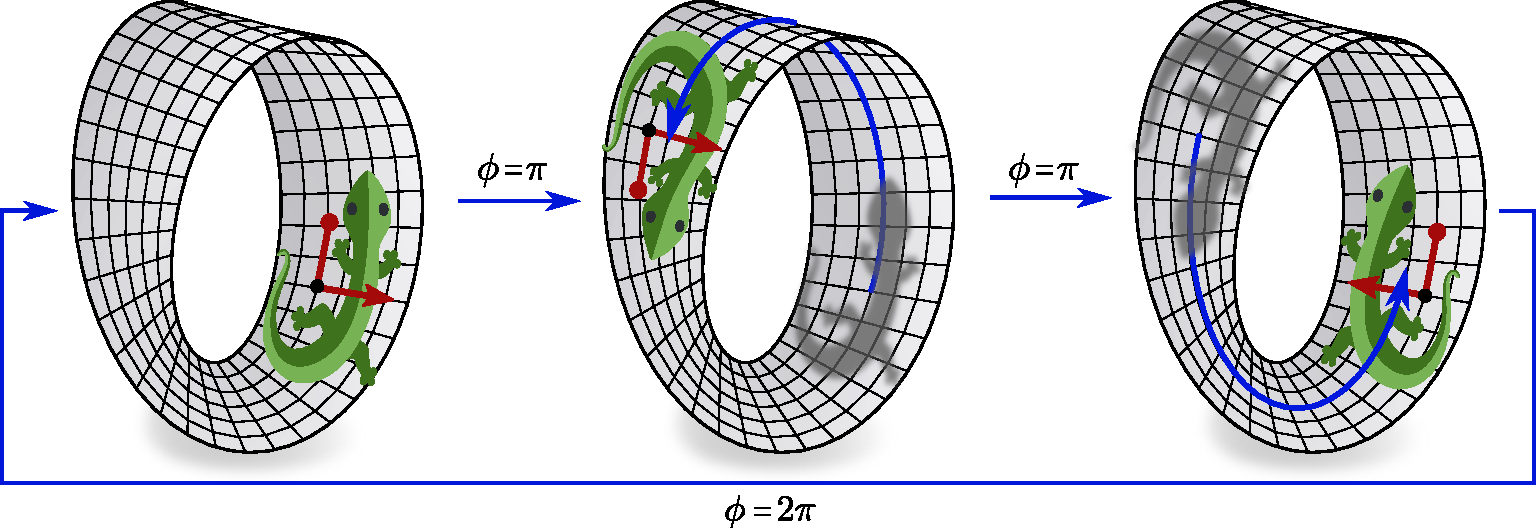
\includegraphics[width=\columnwidth]{figures/mobius_conv_isom.pdf}
	\caption{\small
		تجسم گروه ایزومتری‌های حافظ $\Flip$-ساختار $\IsomRM$ نوار موبیوس که با~$\SO2$ یکریخت است.
		این گروه شامل تمام چرخش‌ها در امتداد نوار است.
		به دلیل پیچ، چرخش $2\pi$، یعنی یک‌بار در اطراف نوار، هنوز آن را به خودش بازنمی‌گرداند بلکه منجر به انعکاس می‌شود.
		پس از دومین دور، یعنی چرخش کل $4\pi$، نوار به خودش بازمی‌گردد.
		تبدیل‌های گیج القا شده مقادیر در $\Flip$ می‌گیرند.
		{
			\\ \color{gray} \scriptsize
			(مارمولک‌ها تحت مجوز \lr{Creative Commons Attribution 4.0 International}
			\href{https://github.com/twitter/twemoji/blob/gh-pages/LICENSE-GRAPHICS}{\underline{\lr{license}}}
			با مجوز \lr{Twitter} اقتباس شده‌اند.)
		}
	}
	\label{fig:mobius_conv_isometries}
\end{figure}





%!TEX root=../GaugeCNNTheory.tex

\subsection{میدان‌های ویژگی مستقل از جهت‌گیری}
\label{sec:mobius_representations}

اصل کوواریانس مستلزم آن است که میدان‌های ویژگی روی نوار موبیوس مستقل از مختصات $\RM$ باشند، یعنی آنها باید به‌طور معادل نسبت به چارچوب‌های هر دو دست‌گردی قابل بیان باشند.
بنابراین آنها با انتخاب نمایش گروهی $\rho: \Flip \to \GL{c}$ از گروه انعکاس مشخص می‌شوند که تبدیل بردارهای ویژگی عددی هنگام تعویض بین دو جهت‌گیری را مشخص می‌کند.
در ادامه چند انتخاب ممکن از چنین انواع میدان‌هایی را مورد بحث قرار خواهیم داد.
خواننده ممکن است بخواهد بررسی کند که نمایش‌های پیشنهادی واقعاً همومورفیسم‌های گروهی هستند که $\rho(gh) = \rho(g)\rho(h)\,\ \forall\, g,h\in \Flip$ را برآورده می‌کنند، همانطور که در بخش~\ref{sec:feature_fields} و پاورقی~\ref{footnote:repr_group_homomorphism} خواسته شده است.

ابتدایی‌ترین مثال، که برای هر گروه ساختار وجود دارد، \emph{نمایش بدیهی} است
\begin{align}
	\rhotriv: \Flip \to \GL{1}\ , \qquad 
	\begin{aligned}
		e &\mapsto \big[\mkern2mu 1 \mkern2mu\big] \\[2pt]
		s &\mapsto \big[\mkern2mu 1 \mkern2mu\big] \\
	\end{aligned}
	\quad ,
\end{align}
که ماتریس همانی ${1\!\times\!1}$ را به هر دو عنصر گروه اختصاص می‌دهد.
این میدان‌های اسکالر $f_{\textup{triv}}$ را مدل می‌کند که از بردارهای ویژگی یک‌بعدی تشکیل شده‌اند که مختصات‌سازی‌های آنها $f^A_{\textup{triv}}(p) \in \R^1$ \emph{تحت انعکاس‌های چارچوب نامتغیر باقی می‌مانند}.
دومین نمایش یک‌بعدی، \emph{نمایش تغییر علامت} است
\begin{align}
	\rhosign: \Flip \to \GL{1}\ , \qquad 
	\begin{aligned}
		e &\mapsto \big[\mkern2mu 1 \mkern2mu\big] \\[2pt]
		s &\mapsto \big[\! \shortminus\!1 \big]
	\end{aligned}
	\quad .
\end{align}
این ماتریس همانی منفی ${1\!\times\!1}$ را به انعکاس‌ها اختصاص می‌دهد و بنابراین میدان‌های شبه‌اسکالر را توصیف می‌کند، یعنی میدان‌های ویژگی یک‌بعدی $f_{\textup{sign}}$ که ضرایب عددی آنها $f^A_{\textup{sign}}(p) \in \R^1$ \emph{تحت انعکاس‌ها علامت خود را تغییر می‌دهند}، \mbox{یعنی} ${\rhosign(s)\cdot f^A_{\textup{sign}}(p) = -f^A_{\textup{sign}}(p)}$.
از آنجا که نمایش بدیهی و نمایش تغییر علامت یک‌بعدی هستند، هر دو نمایش‌های غیرقابل کاهش (\lr{irreps}) گروه انعکاس هستند.
در واقع، آنها تنها دو \lr{irrep} گروه انعکاس هستند.%
\footnote{
	گروه انعکاس با گروه دوری $\Z/2\Z$ از مرتبه دو یکریخت است.
	به خوبی شناخته شده است که \lr{irrep}های گروه‌های دوری از مرتبه $N$ متناظر با ریشه‌های $N$ام وحدت هستند که برای $N=2$ فقط $+1$ (بدیهی) و $-1$ (تغییر علامت) هستند.
}

از آنجا که $\Flip$ گروه متناهی است، نمایش \emph{منظم} متناهی‌بعدی (دوبعدی) دارد
\begin{align}
	\rhoreg: \Flip \to \GL{2}\ , \qquad 
	\begin{aligned}
		e &\mapsto
		\begin{bmatrix} \hspace{1.5pt}
			1 &\mkern-4mu 0 \hspace*{1.5pt} \\ \hspace{1.5pt} 0 &\mkern-4mu 1 \hspace*{1.5pt}
		\end{bmatrix} \\[2pt]
		s &\mapsto 
		\begin{bmatrix} \hspace{1.5pt}
			0 &\mkern-4mu 1 \hspace*{1.5pt} \\ \hspace{1.5pt} 1 &\mkern-4mu 0 \hspace*{1.5pt}
		\end{bmatrix}
	\end{aligned}
	\quad ,
\end{align}
که عناصر گروه را توسط ماتریس‌های جایگشت نمایش می‌دهد.
طبق تعریف، نمایش منظم جایگشت عناصر گروه در $\Flip$ هنگام عمل بر خودشان را مدل می‌کند.
این را با ستون‌های جدول ضرب در معادله~\eqref{eq:reflection_multiplication_table} مقایسه کنید:
ستون میانی را می‌توان به‌عنوان ناشی از عمل $\rhoreg(e)$ بر ستون چپ در نظر گرفت، در حالی که عناصر گروه جابه‌جا شده در ستون راست متناظر با جایگشت توصیف شده توسط عمل $\rhoreg(s)$ بر ستون چپ هستند.
میدان‌های ویژگی منظم $f_{\textup{reg}}$ از $\Flip$ به‌طور عددی توسط بردارهای ویژگی دوبعدی $f^A_{\textup{reg}}(p) \in \R^2$ نمایش داده می‌شوند که دو \emph{کانال آنها تحت انعکاس‌ها جابه‌جا می‌شوند}، یعنی
$
\rhoreg(s) \mkern-1mu\cdot\mkern-2mu f^A_{\textup{reg}}(p)
\,=\,
\begin{bmatrix} \hspace{1.5pt} 0 &\mkern-4mu 1 \hspace*{1.5pt} \\ \hspace{1.5pt} 1 &\mkern-4mu 0 \hspace*{1.5pt} \end{bmatrix}
\mkern-4mu \cdot\mkern-4mu 
\begin{bmatrix} f^A_{\textup{reg},1} \\ f^A_{\textup{reg},2} \end{bmatrix} \!(p)
\,=\,
\begin{bmatrix} f^A_{\textup{reg},2} \\ f^A_{\textup{reg},1} \end{bmatrix} \!(p)
$.

نمایش منظم قابل کاهش است، یعنی شامل دو زیرفضای نامتغیر حقیقی است که در این مورد متناظر با نمایش بدیهی و نمایش تغییر علامت هستند.
بنابراین می‌توان آن را به‌طور معادل به‌عنوان ساخته شده از مجموع مستقیم $\rhotriv \oplus \rhosign$ آن دو \lr{irrep} و تغییر پایه $Q$ در نظر گرفت:
\begin{align}\label{eq:rho_reg_decomposition}
	\rhoreg(g)\ =\ Q\, \big( \rhotriv \!\oplus\mkern-1mu \rhosign \big)\mkern-2mu(g)\; Q^\top
	\quad\ \textup{که در آن } \quad
	Q = \frac{1}{\sqrt{2}}
	\begin{bmatrix} \hspace{1.5pt}
		1 &\mkern-7mu \shortminus1 \hspace*{1.5pt} \\ \hspace{1.5pt} 1 &\mkern-7mu \phantom{\shortminus}1 \hspace*{1.5pt}
	\end{bmatrix}
\end{align}
اعتبار این گزاره به‌آسانی با جایگذاری سمت راست برای هر دو عنصر گروه تأیید می‌شود:
\begin{align}
	Q\, \big( \rhotriv \!\oplus\mkern-1mu \rhosign \big)\mkern-2mu(e)\; Q^\top
	\ =\ \frac{1}{2}
	\begin{bmatrix} \hspace{1.5pt}
		1 &\mkern-7mu \shortminus1 \hspace*{1.5pt} \\ \hspace{1.5pt} 1 &\mkern-7mu \phantom{\shortminus}1 \hspace*{1.5pt}
	\end{bmatrix} \mkern-6mu \cdot\mkern-6mu
	\begin{bmatrix} \hspace{1.5pt}
		1 &\mkern-7mu 0 \hspace*{1.5pt} \\ \hspace{1.5pt} 0 &\mkern-7mu 1 \hspace*{1.5pt}
	\end{bmatrix} \mkern-6mu \cdot\mkern-6mu
	\begin{bmatrix} \hspace{1.5pt}
		\phantom{\shortminus}1 &\mkern-7mu 1 \hspace*{1.5pt} \\ \hspace{1.5pt} \shortminus1 &\mkern-7mu 1 \hspace*{1.5pt}
	\end{bmatrix}
	\ =\ 
	\begin{bmatrix} \hspace{1.5pt}
		1 &\mkern-7mu 0 \hspace*{1.5pt} \\ \hspace{1.5pt} 0 &\mkern-7mu 1 \hspace*{1.5pt}
	\end{bmatrix}
	\ =\ \rhoreg(e)
\end{align}
\begin{align}
	Q\, \big( \rhotriv \!\oplus\mkern-1mu \rhosign \big)\mkern-2mu(s)\; Q^\top
	\,=\, \frac{1}{2}
	\begin{bmatrix} \hspace{1.5pt}
		1 &\mkern-7mu \shortminus1 \hspace*{1.5pt} \\ \hspace{1.5pt} 1 &\mkern-7mu \phantom{\shortminus}1 \hspace*{1.5pt}
	\end{bmatrix} \mkern-6mu \cdot\mkern-6mu
	\begin{bmatrix} \hspace{1.5pt}
		1 &\mkern-7mu \phantom{\shortminus}0 \hspace*{1.5pt} \\ \hspace{1.5pt} 0 &\mkern-7mu \shortminus1 \hspace*{1.5pt}
	\end{bmatrix} \mkern-6mu \cdot\mkern-6mu
	\begin{bmatrix} \hspace{1.5pt}
		\phantom{\shortminus}1 &\mkern-7mu 1 \hspace*{1.5pt} \\ \hspace{1.5pt} \shortminus1 &\mkern-7mu 1 \hspace*{1.5pt}
	\end{bmatrix}
	\,=\, \frac{1}{2}
	\begin{bmatrix} \hspace{1.5pt}
		1 &\mkern-7mu \phantom{\shortminus}1 \hspace*{1.5pt} \\ \hspace{1.5pt} 1 &\mkern-7mu \shortminus1 \hspace*{1.5pt}
	\end{bmatrix} \mkern-6mu \cdot\mkern-6mu
	\begin{bmatrix} \hspace{1.5pt}
		\phantom{\shortminus}1 &\mkern-7mu 1 \hspace*{1.5pt} \\ \hspace{1.5pt} \shortminus1 &\mkern-7mu 1 \hspace*{1.5pt}
	\end{bmatrix}
	\,=\, 
	\begin{bmatrix} \hspace{1.5pt}
		0 &\mkern-7mu 1 \hspace*{1.5pt} \\ \hspace{1.5pt} 1 &\mkern-7mu 0 \hspace*{1.5pt}
	\end{bmatrix}
	\,=\, \rhoreg(s)
\end{align}
به‌طور کلی‌تر، هر نمایش متناهی‌بعدی گروه‌های فشرده (از جمله متناهی) \emph{کاملاً قابل کاهش} به مجموع مستقیم \lr{irrep}ها است~\cite{gallier2019harmonicRepr,din2017reprLectureNotes,serre1977linear}.
این نشان می‌دهد که هر بردار ویژگی کوواریانت که تحت گروه ساختار فشرده تبدیل می‌شود، تا حد تغییر پایه می‌تواند از ویژگی‌های \lr{irrep} ساخته شود.
همانطور که در~\cite{Weiler2019_E2CNN} استدلال شده است، در این مورد واقعاً امکان کاهش هر عملیات شبکه \emph{خطی} به عملیات معادل بین میدان‌های \lr{irrep} وجود دارد که ساخت فضای کرنل‌های $G$-راهبری‌پذیر در معادله~\eqref{eq:G-steerable_kernel_space} و بایاس‌های نامتغیر در معادله~\eqref{eq:gauge_bias_solution_space} را ساده می‌کند.
با این حال، همانطور که در ادامه خواهیم دید، انتخاب خاص پایه از انواع میدان معادل تأثیر کاملاً قابل توجهی بر عملکرد مدل دارد.
دلیل این امر آن است که عملیات شبکه \emph{غیرخطی} به پایه انتخاب شده حساس هستند، یعنی به انتخاب خاصی از انواع میدان معادل.

%!TEX root=../GaugeCNNTheory.tex

\subsection{شبکه‌های کانولوشنی مستقل از جهت‌گیری}
\label{sec:mobius_cnn_ops_analytical}

برای ساخت \lr{CNN}های مستقل از جهت‌گیری روی نوار موبیوس باید لایه‌های هم‌متغیر گیج از بخش~\ref{sec:gauge_CNNs_local} را برای گروه انعکاس~$\Flip$ نمونه‌سازی کنیم.
به‌طور مشخص‌تر، هر یک از توابع الگوی مشترک هم‌متغیر که لایه‌های مستقل از جهت‌گیری را تعریف می‌کنند باید برای هر انتخاب از انواع میدان در نظر گرفته شده $\rhotriv$، $\rhosign$ و $\rhoreg$ نمونه‌سازی شوند.
بخش~\ref{sec:mobius_bias} در ادامه با حل فضاهای $\mathscr{B}^R_\rho$ الگوهای بایاس نامتغیر گیج از معادله~\eqref{eq:gauge_bias_solution_space} شروع می‌کند.
چند انتخاب مجاز از غیرخطی‌های هم‌متغیر گیج برای انواع میدان مختلف در بخش~\ref{sec:mobius_nonlin} پیشنهاد می‌شوند.
بخش~\ref{sec:mobius_kernel_spaces} سپس فضاهای $\KR$ کرنل‌های $\Flip$-راهبری‌پذیر (معادله~\eqref{eq:G-steerable_kernel_space}) را برای هر جفت ممکن از \lr{irrep}های ورودی و خروجی استخراج خواهد کرد.
در حالی که این بخش عمدتاً شامل اشتقاقات نظری خواهد بود، بخش~\ref{sec:mobius_experiment_main} در ادامه جزئیات پیاده‌سازی عملی‌تری را پوشش خواهد داد.

\subsubsection{جمع بایاس مستقل از جهت‌گیری}
\label{sec:mobius_bias}

فضای الگوهای بایاس که می‌توانند به میدانی از نوع $\rho$ بدون دخالت در فرض استقلال از مختصات جمع شوند، در بخش~\ref{sec:gauge_bias_summation} نشان داده شد که توسط
\begin{align}
	\mathscr{B}^{\Flip}_\rho\ :=\ \big\{ b \in\R^c \;\big|\; b = \rho(g)\mkern2mu b\ \ \ \forall g\in \Flip \big\} \,.
\end{align}
داده می‌شود.
برای مورد گروه انعکاس، فقط دو عنصر گروه و بنابراین دو قید وجود دارد.
قید برای عنصر همانی $g=e$ به‌طور بدیهی برآورده می‌شود زیرا $\rho(e) = \id_{\R^c}$ طبق تعریف همیشه همانی روی~$\R^c$ است.
در ادامه بنابراین کافی است توجه را به قید $b = \rho(s)\mkern2mu b$ ناشی از انعکاس $g=s$ محدود کنیم.

با مورد میدان‌های اسکالر، یعنی نمایش بدیهی، شروع می‌کنیم.
قید انعکاس سپس $b = \rhotriv(s)\mkern2mu b = b$ می‌شود که همیشه برآورده می‌شود.
نتیجه می‌شود که فضای الگوهای بایاس
\begin{align}
	\mathscr{B}^{\Flip}_{\scalebox{.8}{$\rho_{{\textup{triv}}}$}} = \R
\end{align}
بدون قید باقی می‌ماند به‌طوری که بایاس‌های دلخواه با مقدار حقیقی می‌توانند به میدان‌های اسکالر جمع شوند.
برای نمایش تغییر علامت، قید انعکاس به $b = \rhotriv(s)\, b = -b$ تبدیل می‌شود و بنابراین فقط برای بایاس‌هایی که صفر هستند برآورده می‌شود:
\begin{align}
	\mathscr{B}^{\Flip}_{\scalebox{.8}{$\rho_{{\textup{sign}}}$}} = \{0\}
\end{align}
بنابراین جمع بایاس به میدان‌های تغییر علامت با حفظ استقلال از مختصات غیرممکن است.
سومین نوع میدان نمونه ما نمایش منظم دوبعدی است.
قید انعکاسی متناظر روی $b\in\R^2$ به صورت زیر است
\begin{align}
	\begin{bmatrix} b_1 \\ b_2 \end{bmatrix}
	\ =\ 
	b
	\ =\ 
	\rhoreg(s)\mkern2mu b
	\ =\ 
	\begin{bmatrix} \hspace{1.5pt}
		0 &\mkern-7mu 1 \hspace*{1.5pt} \\ \hspace{1.5pt} 1 &\mkern-7mu 0 \hspace*{1.5pt}
	\end{bmatrix}
	\!\cdot\! \begin{bmatrix} b_1 \\ b_2 \end{bmatrix}
	\ =\ 
	\begin{bmatrix} b_2 \\ b_1 \end{bmatrix}
\end{align}
و به فضای حل یک‌بعدی منجر می‌شود
\begin{align}\label{eq:bias_solution_space_regular}
	\mathscr{B}^{\Flip}_{\scalebox{.8}{$\rho_{{\textup{reg}}}$}} = 
	\big\{ b\in\R^2 \,\big|\, b_1=b_2 \big\} =
	\bigg\{ \begin{bmatrix} \beta \\ \beta \end{bmatrix} \,\bigg|\, \beta\in\R \bigg\} \ .
\end{align}
استقلال از مختصات این قید به‌طور شهودی روشن است:
از آنجا که نمایش منظم دو کانالی که میدان را تشکیل می‌دهند جابه‌جا می‌کند، جمع بایاس تنها زمانی مستقل از مختصات است که مقادیر جمع شده به هر دو کانال برابر باشند، به‌طوری که ترتیب آنها اهمیت نداشته باشد.

همانطور که قبلاً در بخش~\ref{sec:gauge_bias_summation} ادعا شد، فضای حل $\mathscr{B}^{\Flip}_\rho$ برای نمایش $\rho$ دقیقاً با زیرنمایش‌های بدیهی آن منطبق است.
این مطمئناً برای نمایش بدیهی صادق است که می‌توان هر بایاسی را به آن جمع کرد، و نمایش تغییر علامت که خود هیچ زیرنمایش بدیهی ندارد و بنابراین اصلاً بایاس نمی‌پذیرد.
مثال جالب‌تر نمایش منظم است که در معادله~\ref{eq:rho_reg_decomposition} نشان داده شد به مجموع مستقیم نمایش بدیهی و نمایش تغییر علامت تجزیه می‌شود.
فضای حل یک‌بعدی در معادله~\ref{eq:bias_solution_space_regular} دقیقاً متناظر با تک زیرنمایش بدیهی موجود در~$\rhoreg$ است.
برای بررسی اعتبار این گزاره، توجه کنید که بایاس‌های مجاز برای نمایش مجموع مستقیم $\rhotriv \oplus \rhosign$ از شکل $(\beta,\mkern1mu 0\mkern1mu)^\top$ هستند، که در آن $\beta\in\R$.
این نتیجه می‌تواند از طریق تغییر پایه $Q$ به نمایش منظم برگردانده شود که واقعاً حل ما در معادله~\eqref{eq:bias_solution_space_regular} را بازیابی می‌کند:
\begin{align}
	Q \cdot\mkern-2mu \begin{bmatrix} \beta \\ 0 \end{bmatrix}
	\ \propto\ 
	\begin{bmatrix} \hspace{1.5pt}
		1 &\mkern-7mu \shortminus1 \hspace*{1.5pt} \\ \hspace{1.5pt} 1 &\mkern-7mu \phantom{\shortminus}1 \hspace*{1.5pt}
	\end{bmatrix}
	\!\cdot\! \begin{bmatrix} \beta \\ 0 \end{bmatrix}
	\ =\ 
	\begin{bmatrix} \beta \\ \beta \end{bmatrix}
\end{align}